\documentclass{article}
\usepackage{listings}
\usepackage{color}
\usepackage{keyval}
\definecolor{dkgreen}{rgb}{0,0.6,0}
\definecolor{gray}{rgb}{0.5,0.5,0.5}
\definecolor{mauve}{rgb}{0.58,0,0.82}
\usepackage{bookmark}
\usepackage{amsmath}
\usepackage{geometry}
\usepackage{hyperref}
\usepackage{listings}
\usepackage{xcolor}
\usepackage{graphicx}
\usepackage{amsfonts}

\lstset{
  basicstyle=\footnotesize, 
  numbers=left, 
  numberstyle=\tiny\color{gray}, 
  stepnumber=1,
  numbersep=5pt, 
  backgroundcolor=\color{white},
  showspaces=false,
  showstringspaces=false,
  showtabs=false,
  frame=shadowbox,
  rulecolor=\color{black},
  tabsize=2,
  captionpos=b,
  breaklines=true, 
  breakatwhitespace=false, 
  title=\lstname,
  keywordstyle=\color{blue},
  commentstyle=\color{dkgreen},
  escapeinside={\%*}{*)}, 
  morekeywords={*,...} 
}

\begin{document}

To compare the performace of different shortest path algorithms, I generated grids in sizes of 100-1000, with a step of 100, and for each size there will be 5 different layouts of matrices generated. The following figure shows the performace of the algorithms for different scales on the size of arrays.

\begin{figure}[htbp]
        \centering
        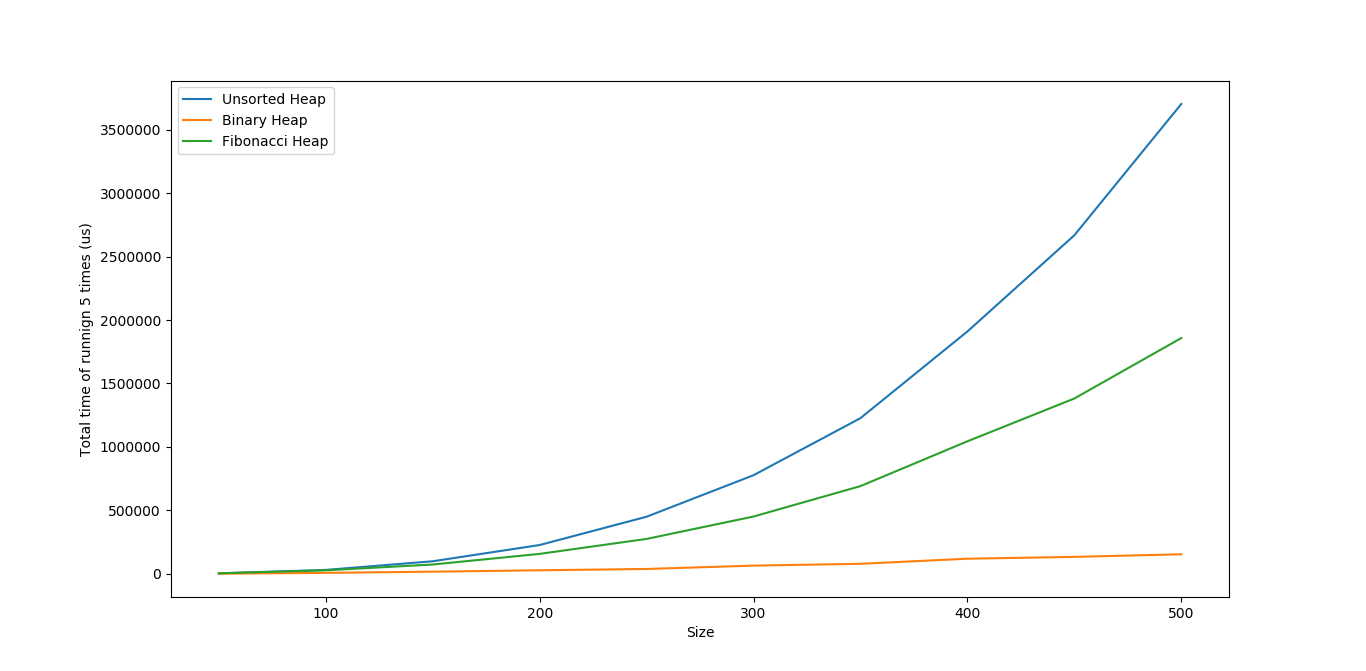
\includegraphics[scale=0.5]{1.png}
\end{figure}

It can be seen that the curve for the unsorted array implementation of priority queue is extremely high. This fact makes sense as the complexity of every operation concerned with minimum value to that implementation will cost $\mathcal{O}(n)$ time, so it is really not a good choice in implementing a priority queue.

As for the Fibonacci heap implementation of the priority queue, although most of the operations on it is under an $\mathcal{O}(1)$ time in amortized consideration, but the constant coefficient is much high, which lead to the phenomenon that the performance of it is slow. However, when the size of the grid grows to extremely large values, the performance of it is expected to be higher.

The binary heap implementation of the priority queue works very fast in practice, and it is because that the complexity of its operations is much lower than unsorted array and it does not have a large constant coefficient like Fibonacci Heap.

The source code are attached in the pages following. The main code and the code for testing are in the same file, but called with different compile option, so the code for comparing is also in the appendix.

\newpage

{\bf 1. Source Code for algorithms and main function.}
\begin{lstlisting}[title=main.cpp,language=C++]
#include "path.h"
#include "string"
#include<cstdlib>
#ifdef P3_CLOCK
#include <ctime>
#include <sys/time.h>
#endif

#ifndef P3_CLOCK
int main(int argc, char *argv[]){
    std::ios::sync_with_stdio(false);
    std::cin.tie(0);
    long int m,n;
    long int sx,sy,ex,ey;
    Modes mode;
    bool v = false;
    std::string ms[3] = {"UNSORTED","BINARY","FIBONACCI"};
    for (long int i=0;i<argc;i++){
        if ((std::string(argv[i])=="-i")||(std::string(argv[i])=="--implementation")){
            for (long int j=0;i<3;j++){
                if (std::string(argv[i+1])==ms[j]){
                    mode = Modes(j);
                    break;
                }
            }
        }
        v = v||(std::string(argv[i])=="-v")||(std::string(argv[i])=="--verbose");
    }
    std::cin >> n >> m >> sx >> sy >> ex >> ey;
    point_t **map = new point_t*[m];
    for (long int i=0;i<m;i++){
        map[i] = new point_t[n];
        for (long int j=0;j<n;j++){
            map[i][j].pathcost=0;
            map[i][j].x=j;
            map[i][j].y=i;
            map[i][j].pre=NULL;
            map[i][j].reached=false;
            std::cin >> map[i][j].weight;
        }
    }
    path(m,n,map,sx,sy,ex,ey,mode,v);
    for (long int i=0;i<m;i++) delete []map[i];
    delete []map;
    return 0;
}
#else
int main(){
    srand(time(NULL));
    struct timeval t1,t2;
    long int sizes[10];
    long int ts[3][10];
    for (long int i=0;i<10;i++) {
        sizes[i] = 100*(i+1);
        for (long int j=0;j<3;j++) ts[j][i]=0;
    }
    for (long int i=0;i<10;i++){
        std::cerr << "Size: " << sizes[i]<< std::endl;
        point_t **map = new point_t*[sizes[i]];
        for (long int j=0;j<sizes[i];j++){
            map[j] = new point_t[sizes[i]];
        }
        for (long int j=0;j<5;j++){
            for (long int k=0;k<sizes[i];k++)
                for (long int m=0;m<sizes[i];m++) {
                    map[k][m].weight=mrand48();
                    map[k][m].pathcost=0;
                    map[k][m].pre=NULL;
                    map[k][m].x=m;
                    map[k][m].y=k;
                    map[k][m].reached=false;
                }
            gettimeofday(&t1,NULL);
            path(sizes[i],sizes[i],map,0,0,sizes[i]-1,sizes[i]-1,UNSORTED,false);
            gettimeofday(&t2,NULL);
            ts[0][i]+=(t2.tv_usec-t1.tv_usec)+1000000*(t2.tv_sec-t1.tv_sec);
            for (long int k=0;k<sizes[i];k++)
                for (long int m=0;m<sizes[i];m++) {
                    map[k][m].pathcost=0;
                    map[k][m].reached=false;
                    map[k][m].pre=NULL;
                }
            gettimeofday(&t1,NULL);
            path(sizes[i],sizes[i],map,0,0,sizes[i]-1,sizes[i]-1,BINARY,false);
            gettimeofday(&t2,NULL);
            ts[1][i]+=(t2.tv_usec-t1.tv_usec)+1000000*(t2.tv_sec-t1.tv_sec);
            for (long int k=0;k<sizes[i];k++)
                for (long int m=0;m<sizes[i];m++) {
                    map[k][m].pathcost=0;
                    map[k][m].reached=false;
                    map[k][m].pre=NULL;
                }
            gettimeofday(&t1,NULL);
            path(sizes[i],sizes[i],map,0,0,sizes[i]-1,sizes[i]-1,FIBONACCI,false);
                gettimeofday(&t2,NULL);
            ts[2][i]+=(t2.tv_usec-t1.tv_usec)+1000000*(t2.tv_sec-t1.tv_sec);
        }
        for (long int k=0;k<sizes[i];k++) delete []map[k];
        delete []map;
    }
    for (int i=0;i<3;i++){
        for (int j=0;j<10;j++) std::cout << ts[i][j] <<" ";
        std::cout << std::endl;
    }
    return 0;
}
#endif

\end{lstlisting}
\begin{lstlisting}[title=path.h,language=C++]
#ifndef PATH_H
#define PATH_H
//#define P3_CLOCK
#include "priority_queue.h"
#include "binary_heap.h"
#include "fib_heap.h"
#include "unsorted_heap.h"
#include <iostream>

enum Modes{UNSORTED,BINARY,FIBONACCI,MODES_NUM};

typedef struct __point__{
    long int x,y;
    long int weight;
    long int pathcost;
    bool reached;
    struct __point__ *pre;
}point_t;

struct compare_point{
    bool operator()(const point_t &a,const point_t &b) const{
        if (a.pathcost!=b.pathcost) return a.pathcost<b.pathcost;
        if (a.x!=b.x) return a.x<b.x;
        return a.y<b.y;
    }
};

void path(long int m,long int n, point_t **map,long int sx,long int sy,long int ex,long int ey,Modes mode,bool v);

void backtrace(point_t **map, long int ex,long int ey);
#endif

\end{lstlisting}
\begin{lstlisting}[title=path.cpp,language=C++]
#include "path.h"
void path(long int m,long int n, point_t **map,long int sx,long int sy,long int ex,long int ey,Modes mode,bool v){
    long int direct[4][2] = {{1,0},{0,1},{-1,0},{0,-1}};
    map[sy][sx].pathcost = map[sy][sx].weight;
    map[sy][sx].reached = true;
    priority_queue<point_t,compare_point> *pq;
    switch (mode){
        case UNSORTED:
            pq = new unsorted_heap<point_t,compare_point>;
            break;
        case BINARY:
            pq = new binary_heap<point_t,compare_point>;
            break;
        default:
            pq = new fib_heap<point_t,compare_point>;
            break;            
    }
    pq->enqueue(map[sy][sx]);
    long int counter = 0;
    while (!pq->empty()){
        if (v) std::cout << "Step " << counter << std::endl;
        counter++;
        point_t c = pq->dequeue_min();
        if (v) std::cout << "Choose cell (" << c.x << ", " << c.y << ") with accumulated length " << c.pathcost << ".\n";
        for (long int i=0;i<4;i++){
            long int x1 = c.x+direct[i][0];
            long int y1 = c.y+direct[i][1];
            if (((x1<0)||(y1<0)||(x1>=n)||(y1>=m))||(map[y1][x1].reached)) continue;
            map[y1][x1].pathcost = map[y1][x1].weight+map[c.y][c.x].pathcost;
            map[y1][x1].reached = true;
            map[y1][x1].pre = &(map[c.y][c.x]);
            if ((x1==ex)&&(y1==ey)){
                if (v) std::cout <<  "Cell (" << x1 << ", " << y1 << ") with accumulated length " << map[y1][x1].pathcost << " is the ending point.\n";
#ifndef P3_CLOCK
                std::cout << "The shortest path from (" << sx << ", " << sy << ") to (" << ex << ", " << ey << ") is " << map[y1][x1].pathcost << ".\nPath:\n";
                backtrace(map, ex,ey);
#endif
                delete pq;
                return; 
            } 
            if (v) std::cout << "Cell (" << x1 << ", " << y1 << ") with accumulated length " << map[y1][x1].pathcost << " is added into the queue.\n";
            pq->enqueue(map[y1][x1]);
        }
    }
}

void backtrace(point_t **map, long int ex,long int ey){
    if (map[ey][ex].pre==NULL){
        std::cout << "(" << ex << ", " << ey << ")\n";
        return;
    }
    backtrace(map,map[ey][ex].pre->x,map[ey][ex].pre->y);
    std::cout << "(" << ex << ", " << ey << ")\n";
}

\end{lstlisting}

\end{document}